\frame{
\frametitle{Data in Docker}
We are in a containerized world.\\
Everything is separated.\\
How do we share/access data ?\\
}

\frame{
\frametitle{Data in Docker: Goals}
\begin{itemize}
\item How Docker manages data ?
\item Use different type of data storage
\end{itemize}
}

\frame{
\frametitle{Data in Docker}
Docker has 3 options
\begin{itemize}
\item Volumes
\item Bind Mounts
\item tmpfs mount
\end{itemize}
}


\frame{
\frametitle{Data in Docker}
Docker and data
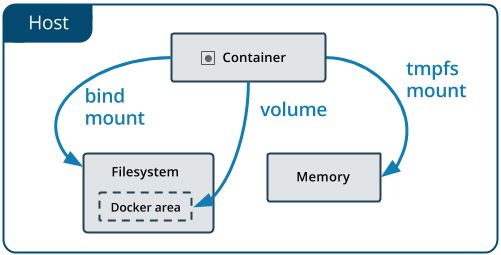
\includegraphics[width=0.50\columnwidth]{./Figure/docker-080-054}
}

\frame{
\frametitle{Data in Docker}
\framesubtitle{Volumes}
\begin{itemize}
\item Managed directly by Docker
\item Saved in \lstinline!/var/lib/docker/volumes/! on the host
\item System processes can not access data outside Docker
\item Recommended by Docker to store data in Docker
\end{itemize}
}

\frame{
\frametitle{Data in Docker}
\framesubtitle{Volumes}

\begin{itemize}
\item User can create its own volumes or instruct Docker to create them when required by the containers or services
\item The container see the volume as a directory and the user define the name
\item Docker guarantees isolation from the host machine
\item A volume can be mounted by many containers at the same time
\end{itemize}
}

\frame{
\frametitle{Data in Docker}
\framesubtitle{Volumes}
\begin{itemize}
\item If not used it is not destroyed, the user must remove the volume explicitly
\item The user can name a volume or Docker create a random name automatically
\item A volume can be an \it{object} in the cloud, the user must use a proper \it{driver}
\item Avoid to increase the size of the container
\end{itemize}
}

\frame{
\frametitle{Data in Docker}
\framesubtitle{Bind mounts}

\begin{itemize}
\item Managed directly by the host OS
\item Saved in  \emph{\color{PineGreen} /in/your/path/} on the host OS
\item System processes or Docker containers can access to the data
\item It is possible to override important files or directory on the host OS
\end{itemize}

}

\frame{
\frametitle{Data in Docker}
\framesubtitle{Bind mounts}

\begin{itemize}
\item Files and directory from the host are mounted inside the container at runtime
\item Require the target's full path on the host machine
\item On demand creation inside the container
\item Very performant
\item Rely on the host filesystem
\item From inside the contianer the user has full access to the filesystem: read/write
\item Read/Write from outside the Docker container
\end{itemize}
}

\frame{
\frametitle{Data in Docker}

Expose a \it{Volume} or \it{Bind Mount} into the container

 \emph{\color{PineGreen} --volume | -v}

Docker infers if it is a \it{Volume} or a \it{Bind Mount} from the command line
}

\frame{
\frametitle{Data in Docker}

In memory storage

 \emph{\color{PineGreen} --tmpfs}

This is useful for ephemeral storage
}

\begin{frame}[fragile]
\frametitle{Data in Docker}
\framesubtitle{When use What}

\begin{itemize}
\item \textit{Volume}
  \begin{itemize}
  \item Sharing data among containers
  \item The host lacks a directory structure
  \item Data can not be stored locally (cloud)
  \end{itemize}
\item \textit{Bind mount}
  \begin{itemize}
  \item Sharing configuration to containers
  \item Sharing source code and build products
  \item Stable directory and file structures shared w/ containers
  \end{itemize}
\end{itemize}
\end{frame}

\begin{frame}[fragile]
\frametitle{Data in Docker}
\framesubtitle{CLI}

\begin{lstlisting}
 docker volume

Commands:
  create   Create a volume
  inspect  Display detailed information on one or more
           volumes
  ls       List volumes
  prune    Remove all unused volumes
  rm       Remove one or more volumes
\end{lstlisting}
\end{frame}


\begin{frame}[fragile]
\frametitle{Data in Docker}
\framesubtitle{Create a volume}

\begin{lstlisting}
$ docker volume create edr19-storage

edr19-storage
\end{lstlisting}
\end{frame}

\begin{frame}[fragile]
\frametitle{Data in Docker}
\framesubtitle{List volumes}


\begin{lstlisting}
$ docker volume ls

DRIVER    VOLUME NAME
local     edr19-storage
\end{lstlisting}
\end{frame}

\begin{frame}[fragile]
\frametitle{Data in Docker}
\framesubtitle{Inspecting a volume}
\begin{lstlisting}[breaklines=true]
$ docker volume inspect edr19-storage

[{
  "CreatedAt": "2019-05-20T18:38+00:00",
  "Driver": "local",
  "Labels": {},
  "Mountpoint": "/var/lib/docker/volumes/edr19-storage/_data",
  "Name": "edr19-storage",
  "Options": {},
  "Scope": "local"
  }]
\end{lstlisting}

\end{frame}

\begin{frame}[fragile]
\frametitle{Data in Docker}
\framesubtitle{Use a volume}

Run a container with Ubuntu 18.04 and create a file with something inside
\begin{lstlisting}
$ docker run --rm \
             -v edr19-storage:/data \
             -it ubuntu:18.04 /bin/bash 
$ echo $RANDOM > /data/seed
$ exit
\end{lstlisting}

After closing the container data are stored an can be accessed
by another container

\begin{lstlisting}
$ docker run --rm \
             -v edr19-storage:/data \
             -it ubuntu:18.04 /bin/bash \
             -c "cat /data/seed"
\end{lstlisting}
\end{frame}

\begin{frame}[fragile]
\frametitle{Data in Docker}
\framesubtitle{Mount points}

Load your own directory inside the container

\begin{lstlisting}
$ docker run -v /opt:/host/opt \
             --name edr19 \
             --rm \
             -it ubuntu:18.04 /bin/bash
\end{lstlisting}
\end{frame}

\begin{frame}[fragile]
\frametitle{Data in Docker}
\framesubtitle{Mount points}

Load your own directory inside the container

\begin{lstlisting}
$ docker run -v /opt:/host/opt \
             --name edr19 \
	      --rm \
            -it ubuntu:18.04 /bin/bash

\end{lstlisting}

\it{Docker does not like relative path}
\end{frame}

\begin{frame}[fragile]
\frametitle{Data in Docker}
\framesubtitle{Volumes and Mount points}

Combine volumes and mount points in a single instance

\begin{lstlisting}
$ docker run -v /opt:/host/opt \
             -v edr19-storage:/data \
             --name edr19 \
             --rm \
             -it ubuntu:18.04 /bin/bash
\end{lstlisting}
\end{frame}

\begin{frame}[fragile]
\frametitle{Data in Docker}
\framesubtitle{Share data w/ containers}


\begin{lstlisting}
$ docker run -v /opt:/host/opt \
             -v edr19-storage:/data \
             --name edr19 \
             --rm \
             -it ubuntu:18.04 /bin/bash

\end{lstlisting}
Another container can access to the data at the same time
\begin{lstlisting}
$ docker run --volumes-from edr19 \
             --name backup \
             --rm \
             -it ubuntu:18.04 /bin/bash
\end{lstlisting}
\it{You may notice some lag in updating data, it depends on the underlying Docker filesystem}
\end{frame}

\begin{frame}[fragile]
\frametitle{Data in Docker}
\framesubtitle{Share data w/ containers}

\scriptsize
\begin{lstlisting}
$ docker run -v /opt:/host/opt \
             -v edr19-storage:/data \
             --name edr19 \
             --rm \
             -it ubuntu:18.04 /bin/bash
\end{lstlisting}
\normalsize
Another container can access to the data and perform a backup automatically
\scriptsize
\begin{lstlisting}
$ docker run --volumes-from edr19 \
             --name backup \
            --rm \
            -it ubuntu:18.04 \
            tar vcz /host/opt/backup.tar.gz /data
\end{lstlisting}
\normalsize
\it{You may notice some lag in updating data, it depends on the underlying Docker filesystem}
\end{frame}

\begin{frame}[fragile]
\frametitle{Data in Docker}
\framesubtitle{Volumes on the fly}

When needed you can even create a Volume at runtime w/o using the explicit \lstinline{create} command. 

\begin{lstlisting}
$ docker run -v bioinfo:/reads \
             -v /opt:/host/opt \
             -v edr19-storage:/data \
             --name edr19 \
             --rm \
             -it ubuntu:18.04 /bin/bash
\end{lstlisting}
\end{frame}

\begin{frame}[fragile]
\frametitle{Data in Docker}
\framesubtitle{Volumes on the fly}

When needed you can even create a Volume at runtime w/o using the explicit \lstinline{create} command. 

\begin{lstlisting}
$ docker volume ls

DRIVER    VOLUME NAME
local     edr19-storage
local     bioinfo
\end{lstlisting}
\end{frame}

\begin{frame}[fragile]
\frametitle{Data in Docker}
\framesubtitle{Anonymous Volumes} 

When needed you can even create a Volume at runtime w/o using the explicit \lstinline{create} command. 

\begin{lstlisting}
$ docker run -v /anonymous \
             -v bioinfo:/reads \
             -v /opt:/host/opt \
             -v edr19-storage:/data \
             --name edr19 \
             --rm \
             -it ubuntu:18.04 /bin/bash
\end{lstlisting}
\end{frame}

\begin{frame}[fragile]
\frametitle{Data in Docker}
\framesubtitle{Anonymous Volumes}

When needed you can even create a Volume at runtime w/o using the explicit \lstinline{create} command. 

\begin{lstlisting}
$ docker volume ls

DRIVER    VOLUME NAME
local     edr19-storage
local     bioinfo
\end{lstlisting}

\it{Once exited from the container, there is no evidence about the anonymous container}
\end{frame}

\begin{frame}[fragile]
\frametitle{Data in Docker}
\framesubtitle{Anonymous Volumes}

w/o \lstinline{--rm}

When needed you can even create a Volume at runtime w/o using the explicit \lstinline!create! command. 


\begin{lstlisting}
$ docker run -v /anonymous \
             -v bioinfo:/reads \
             -v /opt:/host/opt \
             -v edr19-storage:/data \
             --name edr19 \
             -it ubuntu:18.04 /bin/bash
\end{lstlisting}
\end{frame}

\begin{frame}[fragile]
\frametitle{Data in Docker}
\framesubtitle{Anonymous Volumes}
 w/o \lstinline{--rm}

When needed you can even create a Volume at runtime w/o using the explicit \lstinline{create} command. 


\begin{lstlisting}
$ docker volume ls

DRIVER    VOLUME NAME
local     edr19-storage
local     bioinfo
local     8a76g20jc0gcbgf3952gbdnihd253r801skala7898y...
\end{lstlisting}
\end{frame}

\begin{frame}[fragile]
\frametitle{Data in Docker}
\framesubtitle{Tech notes}

Docker \it{volumes}, \it{images}, \it{container} are capped to a defaul value which is configured at daemon level usually around \texttt{10 GB}

\begin{lstlisting}
dm.basesize
\end{lstlisting}
\end{frame}

\frame{
\frametitle{Data in Docker}
\framesubtitle{Tech notes}

The \lstinline{dm.basesize} can be increased but the Docker's daemon must be restared.
}

\begin{frame}[fragile]
\frametitle{Data in Docker}
\framesubtitle{Tech notes}

The user can run the daemon by hand 
\begin{lstlisting}
$ sudo dockerd --storage-opt dm.basesie=50G
\end{lstlisting}
\end{frame}

\frame{
\frametitle{Data in Docker}
\framesubtitle{Tech notes}

The user can increase the size but never decrease it.

If the user specifes a value which is lower than the minimum size of \it{volumes}, \it{images}, \it{containers} Docker will complain with errors.
}

\begin{frame}[fragile]
\frametitle{Data in Docker}
\framesubtitle{Tech notes}

Usually everything works fine, but may happend that Docker' system dir should be wiped out
\begin{lstlisting}
$ sudo service docker stop

$ sudo rm -rf /var/lib/docker
\end{lstlisting}
\end{frame}